\documentclass[10pt]{article}

%AMS-TeX packages
\usepackage{amssymb,amsmath,amsthm} 
%geometry (sets margin) and other useful packages
\usepackage[margin=1.25in]{geometry}
\usepackage{graphicx,ctable,booktabs}
\usepackage{verbatim}
\usepackage{color}
\usepackage{listings}
\lstset{ %
language=C,                % choose the language of the code
basicstyle=\footnotesize,       % the size of the fonts that are used for the code
numbers=left,                   % where to put the line-numbers
numberstyle=\footnotesize,      % the size of the fonts that are used for the line-numbers
stepnumber=1,                   % the step between two line-numbers. If it is 1 each line will be numbered
numbersep=5pt,                  % how far the line-numbers are from the code
backgroundcolor=\color{white},  % choose the background color. You must add \usepackage{color}
showspaces=false,               % show spaces adding particular underscores
showstringspaces=false,         % underline spaces within strings
showtabs=false,                 % show tabs within strings adding particular underscores
frame=single,           % adds a frame around the code
tabsize=2,          % sets default tabsize to 2 spaces
captionpos=b,           % sets the caption-position to bottom
breaklines=true,        % sets automatic line breaking
breakatwhitespace=false,    % sets if automatic breaks should only happen at whitespace
escapeinside={\%*}{*)}          % if you want to add a comment within your code
}

%
%Fancy-header package to modify header/page numbering 
%
\usepackage{fancyhdr}
\pagestyle{fancy}
%\addtolength{\headwidth}{\marginparsep} %these change header-rule width
%\addtolength{\headwidth}{\marginparwidth}
\lhead{CS 261 Project Proposal}
\chead{} 
\rhead{\thepage} 
\lfoot{\small Andrew Johnson and Scott Moore} 
\cfoot{} 
\rfoot{\footnotesize CS 261 Project Proposal} 
\renewcommand{\headrulewidth}{.3pt} 
\renewcommand{\footrulewidth}{.3pt}
\setlength\voffset{-0.25in}
\setlength\textheight{648pt}

\usepackage[square,numbers]{natbib}

%%%%%%%%%%%%%%%%%%%%%%%%%%%%%%%%%%%%%%%%%%%%%%%

\usepackage{trfrac}
\newcommand{\sign}[2]{\ensuremath{#1\;\textsf{signed}\;#2}}
\newcommand{\imp}[2]{\ensuremath{#1 \rightarrow #2}}
\newcommand{\says}[2]{\ensuremath{#1\;\textsf{says}\;#2}}
\newcommand{\confirms}[2]{\ensuremath{#1\;\textsf{confirms}\;#2}}
\newcommand{\ctxt}[0]{\ensuremath{\Gamma}}
\newcommand{\nil}[0]{\ensuremath{\cdot}}
\newcommand{\bnfsep}[0]{\ensuremath{\quad\mid\quad}}
\newcommand{\entails}[2]{\ensuremath{#1 \vdash #2}}
\newcommand{\pred}[2]{\ensuremath{\textsc{#1}(#2)}}
\newcommand{\subst}[2]{\ensuremath{[#1/#2]}}
\newcommand{\abs}[1]{\ensuremath{\forall x:\;#1}}
\newcommand{\rtcheck}[0]{\ensuremath{\textsf{Runtime check}}}
\newcommand{\with}[1]{\ensuremath{\;(\text{with } #1)}}
\newcommand{\todo}[1]{{\color{red}todo: {#1}}}

\begin{document}

\title{Authorization Logic in JOS}
\author{Andrew Johnson and Scott Moore}

\maketitle

\thispagestyle{empty}

\begin{section}{Introduction}
Authorization logics are a principled technique for implementing rule-based access control mechanisms.
They have several advantages over traditional OS access control mechanisms such as access control lists.
In particular, they allow principals to express access control decisions for which they do not have complete information.
Authorization logics also provide \emph{proof-carrying authorization}. That is, the capability to access a resource carries with it the set of authorization decisions that granted it.
\todo{more introduction}

\subsection{Related work}
\todo{more information and reword some}
There has been quite a lot of work on authorization logics, particularly in the context of distributed systems.
Most recently, \citet{Nexus} developed the Nexus operating system, which uses authorization logic to combine different trust bases for secure systems into a cohesive authorization system.
Our system borrows Nexus's authority mechanism to allow revocation and other dynamic authorization policies.

Our authorization logic is based on \citet{Bauer}'s authorization logic extended with a primitive for dynamic authorization checks and cut elimination, which reduces the size of proofs.
More sophisticated authorization logics are given by \citet{AURA} and \citet{Garg}.

\todo{relationship to capabilities}
\end{section}

\begin{section}{Design}

We replaced the current authorization mechanism for jOS system calls (\textsf{envid2env}) with a new mechanism based on authorization logic. Principals (environments) use a secure binding to specify an authorization goal which is used to mediate access to system calls affecting the environment.
An authorization goal is a formula in our authorization logic. Access is granted to any principal presenting a proof of the authorization goal.


Our logic is based on the logic given in \citep{Bauer}, but is similar to the Nexus Authorization Logic (NAL). Like NAL, our logic is constructive, and thus a proof of authorization is also an audit record of the principals and inferences

Our new system uses authorization proofs as capabilities and allows principals 


\todo{rework}
We plan to replace the current authorization mechanism for JOS system calls (\textsf{envid2env}) with a new mechanism based on a simple authorization logic.
Our authorization system will use authorization proofs as capabilities and support dynamic authorization decisions through secure bindings.
Because our authorization library will be implemented primarily in user space, it also provides a mechanism for implementing access control for user level resources.

The principals in our system are environments, \emph{$env_1 \ldots env_n$}.
We believe these are appropriate principals because our authorization decisions apply to system calls, primarily those for manipulating environments.

Our logic is based on the simple logic for access control given in \cite{Bauer}, but extended to support dynamic authorization decisions. The syntax and semantics of the logic are given below and followed with a high level description.
\\[1em]
\begin{tabular}{llcl}
\emph{principals} & R & ::= & $x$ \bnfsep $v$ \\
\emph{predicates} & P & ::= & $pred(R)$ \\
\emph{formulas} & F & ::= & $P$ \bnfsep \imp{F_1}{F_2} \bnfsep \abs{F}\\
                &   & \bnfsep & \sign{A}{F} \bnfsep \says{A}{F} \bnfsep \confirms{A}{F}\\
\emph{contexts} & \ctxt & ::= & \nil \bnfsep \ctxt,$F$ \\
\end{tabular}
{
\center
$\trfrac[\;signed]{\rtcheck}{\entails{\ctxt}{\sign{A}{F}}}$ \hfil
$\trfrac[\;confirms]{\rtcheck}{\entails{\ctxt}{\confirms{A}{F}}}$ \hfil
$\trfrac[\;assump]{F \in \ctxt}{\entails{\ctxt}{F}}$ \\[1em]

$\trfrac[\;tauto]{\entails{\ctxt}{F}}{\entails{\ctxt}{\says{A}{F}}}$ \hfil
$\trfrac[\;weaken impl]{\entails{\ctxt,F_1}{F_2}}{\entails{\ctxt}{\imp{F_1}{F_2}}}$ \hfil
$\trfrac[\;impl]{\entails{\ctxt}{F_1} \quad \entails{\ctxt}{\imp{F_1}{F_2}}}{\entails{\ctxt}{F_2}}$ \\[1em]

$\trfrac[\;sign]{\entails{\ctxt}{\sign{A}{F_1}} \quad \entails{\ctxt,F_1}{\says{A}{F_2}}}{\entails{\ctxt}{\says{A}{F_2}}}$ \hfil
$\trfrac[\;conf]{\entails{\ctxt}{\confirms{A}{F_1}} \quad \entails{\ctxt,F_1}{\says{A}{F_2}}}{\entails{\ctxt}{\says{A}{F_2}}}$ \\[1em]

$\trfrac[\;says]{\entails{\ctxt}{\says{A}{F_1}} \quad \entails{\ctxt,F_1}{\says{A}{F_2}}}{\entails{\ctxt}{\says{A}{F_2}}}$ \hfil
$\trfrac[\;spec]{\entails{\ctxt}{\says{A}{(\abs{F_1})}} \quad \exists p:\;\entails{\ctxt,F_1\subst{p}{x}}{\says{A}{F_2}}}{\entails{\ctxt}{\says{A}{F_2}}}$
}

\medskip

The meta variable $A$ in the formulas \textsf{signed}, \textsf{says} and \textsf{confirms} ranges over principals.
$P$ would denotes uninterpreted first-order predicates (e.g., \pred{Trusted}{Env}, \pred{Parent}{Env}).
The formula \imp{F_1}{F_2} denotes implication. 

\sign{A}{F} indicates that $A$ believes $F$ to be true; at run time, it corresponds to a digitally signed assertion.
\says{A}{F} denotes that $F$ is a statement which $A$ believes given the formulae asserted by A and the beliefs of other principals.

\paragraph{Example} Suppose that principal $A$ wishes to delegate its authorization decisions to $B$. Then $A$ would assert \sign{A}{\imp{(\says{B}{\pred{OK}{Env}})}{\pred{OK}{Env}}}. Now for any principal $C$ authorized by $B$ (\says{B}{\pred{OK}{C}}), we can derive \says{A}{\pred{OK}{C}}.

\medskip

\confirms{A}{F} is a new formula we are adding to the logic and corresponds with the authority abstraction in the Nexus system \cite{Nexus}. 
\confirms{A}{F} is a \emph{secure binding} of a run time authorization decision to a principal. \confirms{A}{F} is validated by invoking a decision procedure in $A$ that takes the authorization formula $F$ as input and returns true if $A$ believes $F$.
Crucially, checking the validity $\confirms{A}{F}$ does not create a reusable proof object.
This allows time-sensitive or revocable authorization decisions to be implemented on top of our simple logic without explicitly incorporating time or revocation as primitives.
\end{section}

\begin{section}{Implementation}
We broke implementation into three stages.  We first embedded our logic into the Coq Proof Assistant.  Second, we ported that code to C as a stand-alone library.  Third, we integrated the library into the JOS operating system.
\subsection{Coq}
In order to ensure the correctness and completeness of our logic and proof checker, we first embedded it into the Coq Proof Assistant.  This enabled us to prove that our proof checker was correct and always terminated, as well as work out some of the implementation details in a strongly typed language.  For example, we first defined variables as strings and carried an environment mapping names to values.  This made the proof checker overly complicated and stripping it out led to a far simpler implementation both in Coq and C.  Writing the proof checker in Coq allowed us to prove that it was correct (in fact, using Coq's dependent types, we actually return the Coq proof that the proof checker is correct from the check function).  We therefore can be assured that we did not skip any corner cases, or over-simplify.  The logic, proof checker, and examples were implemented in about 400 lines in Coq.
\subsection{C Library} \label{sec:clib}
There is no way to directly compile Coq code into C code, so we performed this translation by hand.  This obviously invalidates our proof of correctness.  We gained the fact that our algorithms and data structures were correct, but have no such guarantee for the C implementation.  We attempted to compensate for this by writing a number of tests (now in \textsf{user/proof test.c}).  The C library defines the logic as in section \ref{sec:logic}.  For ease of use we also implemented functions to recursively print formulas and proofs, as well as constructors for primitive proofs, primitive formulas, principals, and for more complex, commonly used, proofs.  
\newline\newline
The context was implemented as a stack of formulas since the proof checker adds a formula to the context and, once it has been used, removes that formula.  Formulas and Proofs are represented as tagged \textsf{union}s of the primitive types together with an \textsf{enum} indicating the current type (another option would be to use C++ subclassing).  To simplify memory management, all constructors perform a deep copy of all input data structures.  This means that a proof can be freed without worry about the constituent subproofs and formulas.  To make this approach easy to implement, each of the data structures has a comparison function and a deep-copy function.  In addition, to ease debugging and introspection, each data structure can be printed as a pre-formatted latex string (many examples of which are in this document).  In total, the library implementation consists of approximately 2600 lines of C, about half of which is test code.
\subsection{JOS Integration}
The library described in section \ref{sec:clib} provides a logic and a method to check proofs defined in that logic.  In order to use this for authorization we needed to integrate it into an operating system.  We chose to use JOS for simplicity; the existing authorization mechanism was easy to replace.  We chose to focus on replacing environment to environment authentication.  In JOS, an environment is authorized to manipulate another only if it is the direct parent environment. We replace this with a more flexible model built on our authorization logic.  Essentially, to manipulate environment A, environment B must provide a proof of a logical formula defined by A.  The modular design of our C library enables us to more or less drop it into JOS as a library.  In order to facilitate this we essentially only needed to implement a JOS memory manager (\textsf{malloc} and \textsf{free}) to replace the \textsf{stdlib} version.
\subsubsection{Environments}
Each environment has the option to define a single logical formula and add a pointer to it to their environment structure.  If environment A defines a formula
\[
F = \says{A}{\pred{OK}{x}}
\]
then $F$ must be proved in order to manipulate $A$.  If environment $B$ has a proof of $F$ then $B$ adds a pointer to this proof in their environment structure before making a system call that would affect environment $A$.  More details on this are presented in the next section.
\subsubsection{System Calls}
If a system call, say \textsf{sys\_page\_map}, will affect a environment $A$ then, when $B$ makes that call, the JOS kernel uses the proof, $P$, that $B$ put into their environment structure and checks that $P$ is a valid proof of the formula, $F$, that $A$ has indicated.  Setting $F$ in $A$ and setting $P$ in $B$ are both accomplished using system calls.  We also add a system call for signing formulas, rather than implementing cryptographic digital signatures.  The kernel stores a list of all signed formulas and checks this list when checking a proof.  See below for a simple example.
\begin{lstlisting}
// Constructed in A

// This is equivalent to [for all x, OK(x)]
// What will actually be proved is [A says OK(B)] where B has been substituted for x
Formula F = formula_pred(OK, x);
sys_set_goal(F);
// Sign formula [B is OK] (this is F with B substituted for x)
sys_sign_formula(formula_subst(F, x, B));

// Constructed in B

// Construct a proof of [A says F(B)]
Formula F_B_subst = formula_pred(OK, B);
Proof P  = says_from_signed(A, F_B_subst);
sys_set_proof(P);
...
// Map a page from B to A
sys_page_map(0, Bvaddr, A, Avaddr, perm);
\end{lstlisting}
\subsubsection{Runtime Verification}
During proof checking there are three runtime checks, context membership, signatures, confirmations.  The first is straightforward and the second is implemented as a special case of the first.  The third, confirmation, relies on code that is defined by the confirming environment.  my making a system call \textsf{sys\_set\_confirms\_upcall} the confirming environment, $A$, can set a function that should be called to check any statement of the form $\confirms{A}{F}$.  At runtime a candidate function is passed into the upcall, which returns a boolean value.  In our implementation we run this code in the proof checker, assuming it is well behaved (terminates, does not abuse privilege).  A future implementation could restrict upcalls to well-behaved functions and check this property at runtime.
\subsubsection{Proof Sharing}
It can be easier to construct a proof or parts of a proof in the environment which defines the goal to be proved.  In these cases the proofs need to be handed out to the provers.  To do this we created library functions to send and receive proofs.  These are implemented on top of IPC, adding handling of dynamically allocated data structures.  We can achieve the same result as above using proof sharing.
\begin{lstlisting}
// Constructed in A
Formula F = formula_pred(OK, x);
sys_set_goal(F);
// This automatically calls sys_sign_formula when called from A
Proof P  = says_from_signed(A, formula_subst(F, x, B));
send_proof(B, P);

// Constructed in B
Proof P = receive_proof();
sys_set_proof(P);
...
// Map a page from B to A
sys_page_map(0, Bvaddr, A, Avaddr, perm);
\end{lstlisting}
\end{section}

\begin{section}{Evaluation}
\subsection{Performance}
\begin{figure}
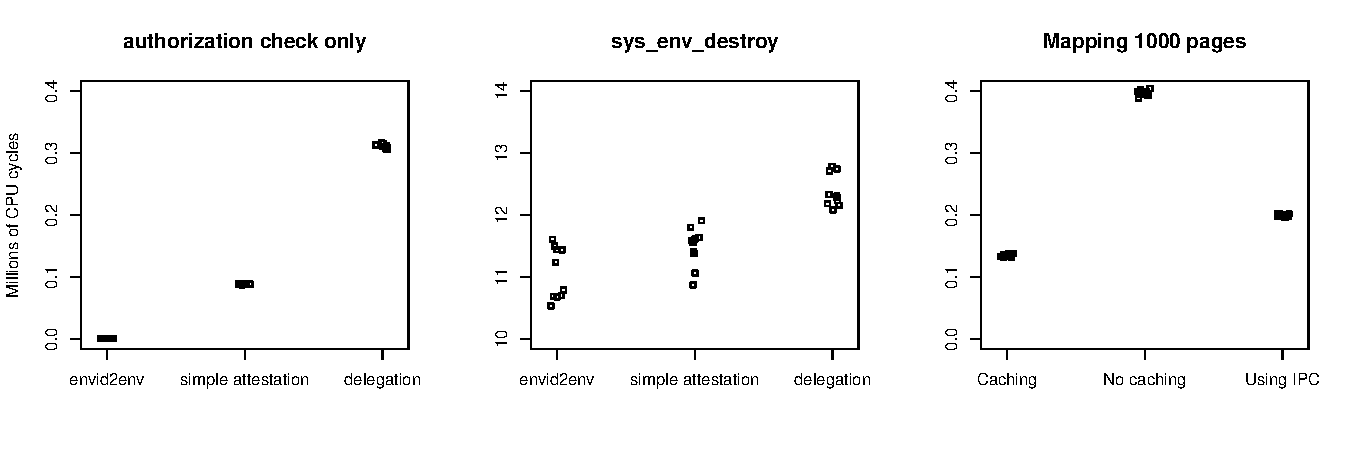
\includegraphics[width=\textwidth]{plots.pdf}
\caption{\todo{caption}}
\label{fig:perf}
\end{figure}

\subsection{Usability}
\end{section}
\begin{section}{Example: Delegation}
Suppose an environment wishes to accept as ``OK'' whatever another environment accepts as ``OK''.  This is a fairly common type of proof called delegation.  Consider the following example.  We have a parent environment, $P$, and two child environments, $C_1$ and $C_2$.
$C_2$ delegates to $P$.  $C_1$ uses this fact along with the fact that $\sign{P}{\pred{OK}{C_1}}$ to prove $\says{C_2}{\pred{OK}{C_1}}$.  This will allow $C_1$ to make system calls affecting $C_2$, such as $\textsf{sys\_page\_map}$.
\newline\newline
$
P_1 = \trfrac[\;sign]{\trfrac[\;signed]{\rtcheck}{\sign{C_2}{\abs{\imp{\says{P}{\pred{OK}{v_{0}}}}{\pred{OK}{v_{0}}}}}} \quad \trfrac[\;tauto]{\trfrac[\;assump]{\rtcheck}{\abs{\imp{\says{P}{\pred{OK}{v_{0}}}}{\pred{OK}{v_{0}}}}}}{\says{C_2}{\abs{\imp{\says{P}{\pred{OK}{v_{0}}}}{\pred{OK}{v_{0}}}}}}}{\says{C_2}{\abs{\imp{\says{P}{\pred{OK}{v_{0}}}}{\pred{OK}{v_{0}}}}}} \\\\\\\\
P_2 = \trfrac[\;tauto]{\trfrac[\;impl]{\trfrac[\;sign]{\trfrac[\;signed]{\rtcheck}{\sign{P}{\pred{OK}{C_1}}} \quad \trfrac[\;tauto]{\trfrac[\;assump]{\rtcheck}{\pred{OK}{C_1}}}{\says{P}{\pred{OK}{C_1}}}}{\says{P}{\pred{OK}{C_1}}} \quad \trfrac[\;assump]{\rtcheck}{\imp{\says{P}{\pred{OK}{C_1}}}{\pred{OK}{C_1}}}}{\pred{OK}{C_1}}}{\says{C_2}{\pred{OK}{C_1}}} \\\\\\\\
\text{DELEGATION} = \trfrac[\;spec]{P_1 \quad C_1 \quad P_2}{\says{C_2}{\pred{OK}{C_1}}} \\\\\\\
$
We have added helper functions to create these proofs.
\begin{lstlisting}
// Constructed in C2
Proof del = delegate_from_signed(C2, P, OK);  

// Constructed in parent
Formula pred = formula_pred(OK, principal_pcpl(C1));
Proof  perm = says_from_signed(P, pred);

// Constructed in C2
Proof  use_del = use_delegation(C2, P, C1, OK, del, perm);
\end{lstlisting}
$P_1$ is a proof that $C_2$ delegates to $P$ for the OK predicate, and is constructed in line 2 above.  $P_2$ begins with $\sign{P}{\pred{OK}{C_1}}$ and is then used together with $P_1$ to prove $\says{C_2}{\pred{OK}{C_1}}$.  There are runtime checks required by ``signed'' to verify the signatures, and by ``assump'' to verify that the given statement is in the context (note that this proof begins with an empty context, but that the proof checker adds to its context at runtime).  
\end{section}

\begin{section}{Future Work}
Kernel principal.
\end{section}

Multiple goals for a single environment.
\begin{section}{Summary}
\end{section}


\bibliographystyle{plainnat}
\bibliography{bib}

\end{document}
